 \documentclass[oneside,11pt]{article}


\usepackage{soul}
\usepackage{natbib}
\usepackage{hyperref}
\usepackage{bookmark}
\usepackage{graphicx}             
\graphicspath{{./Figuras/}}

\usepackage{makecell}
\usepackage[margin=1in]{geometry}
\usepackage{float}                
\usepackage{amsmath}
\usepackage{amscd}
\usepackage{amsfonts}
\usepackage{amssymb}
\usepackage{bbm}
\usepackage{booktabs}
\usepackage{nameref}
\usepackage{multirow}
\usepackage[nokeyprefix]{refstyle}
\usepackage{rotating}
\usepackage{threeparttable}
\usepackage{afterpage}
\usepackage{lscape}
\usepackage{enumerate}
\usepackage{caption}
\usepackage{subcaption}
\usepackage{epstopdf}
\usepackage{setspace}
\usepackage{svg}
\usepackage{dsfont}
\usepackage{amsthm}
\usepackage{tocloft}
\usepackage{etoc}
\usepackage{lmodern}
\usepackage{bm}

\epstopdfDeclareGraphicsRule{.tiff}{png}{.png}{convert #1 \OutputFile}
\AppendGraphicsExtensions{.tiff}

\epstopdfDeclareGraphicsRule{.tif}{png}{.png}{convert #1 \OutputFile}
\AppendGraphicsExtensions{.tif}

\usepackage{tikz}
\usetikzlibrary{shapes.geometric, arrows}
\usetikzlibrary{calc}
\usetikzlibrary{matrix}

\tikzset{ 
    table/.style={
        matrix of nodes,
        row sep=-\pgflinewidth,
        column sep=-\pgflinewidth,
        nodes={
            rectangle,
            draw=black,
            align=center
        },
        minimum height=1.5em,
        text depth=0.5ex,
        text height=2ex,
        nodes in empty cells,
%%
        every even row/.style={
            nodes={fill=gray!20}
        },
        column 1/.style={
            nodes={text width=2em,font=\bfseries}
        },
        row 1/.style={
            nodes={
                fill=black,
                text=white,
                font=\bfseries
            }
        }
    }
}


\usepackage{colortbl}

\newtheorem{theorem}{Theorem}
\newtheorem{claim}[theorem]{Claim}
\newtheorem{prop}[theorem]{Proposition} 
\newtheorem{cor}[theorem]{Corollary} 

\DeclareRobustCommand{\hlgr}[1]{{\sethlcolor{green}\hl{#1}}}


\usepackage{comment}
%para esconder columnas en tablas (enrique)
\usepackage{array}
\newcolumntype{H}{>{\setbox0=\hbox\bgroup}c<{\egroup}@{}}
\linespread{1.25}

\newcommand{\wh}{\widehat}
\usepackage{anyfontsize}

\usepackage[linesnumbered,vlined,ruled,commentsnumbered]{algorithm2e}

\DontPrintSemicolon
\newcommand{\To}{\mbox{\upshape\bfseries to}}
%%% HELPER CODE FOR DEALING WITH EXTERNAL REFERENCES
\usepackage{xr}
\makeatletter
\newcommand*{\addFileDependency}[1]{
  \typeout{(#1)}
  \@addtofilelist{#1}
  \IfFileExists{#1}{}{\typeout{No file #1.}}
}
\makeatother


\newcommand*{\myexternaldocument}[1]{
    \externaldocument{#1}
    \addFileDependency{#1.tex}
    \addFileDependency{#1.aux}
}

%\myexternaldocument{OA}

%%%%%%%%%%%%%%%%%%%%%%%%%%%%%%%% DOCUMENT
\begin{document}

\begin{table}[H]
\caption{Main treatment effects - Financial Cost}
\label{tot_tut}
\begin{center}
\scriptsize{% Table generated by Excel2LaTeX from sheet 'main_te_dec_comparison'
\begin{tabular}{lccccccccccc}
\toprule
      & \multicolumn{3}{c}{FC } &       & \multicolumn{3}{c}{Interest} &       & \multicolumn{3}{c}{Fee} \\
\cmidrule{2-4}\cmidrule{6-8}\cmidrule{10-12}      & (1)   & (2)   & (3)   &       & (4)   & (5)   & (6)   &       & (7)   & (8)   & (9) \\
\midrule
\midrule
Forced-commitment & -389.4*** & -379.7*** & -315.2*** &       & -124.2*** & -157.3*** & -140.3*** &       & 32.4*** & 32.1*** & 31.0*** \\
      & (117.8) & (111.4) & (117.5) &       & (40.0) & (34.9) & (38.1) &       & (1.54) & (1.43) & (1.69) \\
Choice-commitment & -75.0 & -84.9 & -48.5 &       & 8.16  & -24.9 & -17.5 &       & 1.60*** & 1.34** & 1.55*** \\
      & (117.0) & (114.6) & (120.6) &       & (49.5) & (38.4) & (39.3) &       & (0.29) & (0.54) & (0.58) \\
      &       &       &       &       &       &       &       &       &       &       &  \\
\midrule
Observations & 6304  & 6304  & 4837  &       & 6304  & 6304  & 4837  &       & 6304  & 6304  & 4837 \\
R-sq  & 0.004 & 0.007 & 0.007 &       & 0.005 & 0.022 & 0.022 &       & 0.147 & 0.151 & 0.139 \\
Control Mean & 1851.0 & 1851.0 & 1813.6 &       & 545.9 & 545.9 & 519.8 &       & 0     & 0     & 0 \\
Branch-day FE &       & \checkmark & \checkmark &       &       & \checkmark & \checkmark &       &       & \checkmark & \checkmark \\
Survey subsample &       &       & \checkmark &       &       &       & \checkmark &       &       &       & \checkmark \\
\midrule
\midrule
      &       &       &       &       &       &       &       &       &       &       &  \\
\midrule
      & \multicolumn{3}{c}{Cost of losing pawn} &       & \multicolumn{3}{c}{Capital} &       & \multicolumn{3}{c}{Default} \\
\cmidrule{2-4}\cmidrule{6-8}\cmidrule{10-12}      & (10)  & (11)  & (12)  &       & (13)  & (14)  & (15)  &       & (16)  & (17)  & (18) \\
\midrule
\midrule
Forced-commitment & -297.7*** & -254.5** & -205.9* &       & -1.48 & -0.57 & 0.75  &       & -0.077*** & -0.065*** & -0.067*** \\
      & (114.1) & (104.8) & (112.6) &       & (3.14) & (3.03) & (3.55) &       & (0.025) & (0.023) & (0.025) \\
Choice-commitment & -84.8 & -61.4 & -32.5 &       & -3.73 & -3.98 & -2.78 &       & -0.042* & -0.025 & -0.039* \\
      & (111.5) & (109.2) & (116.9) &       & (2.57) & (2.47) & (2.75) &       & (0.023) & (0.021) & (0.023) \\
      &       &       &       &       &       &       &       &       &       &       &  \\
\midrule
Observations & 6304  & 6304  & 4837  &       & 6304  & 6304  & 4837  &       & 6304  & 6304  & 4837 \\
R-sq  & 0.002 & 0.007 & 0.007 &       & 0.001 & 0.003 & 0.004 &       & 0.004 & 0.013 & 0.015 \\
Control Mean & 1305.1 & 1305.1 & 1293.9 &       & 5.82  & 5.82  & 4.90  &       & 0.44  & 0.44  & 0.45 \\
Branch-day FE &       & \checkmark & \checkmark &       &       & \checkmark & \checkmark &       &       & \checkmark & \checkmark \\
Survey subsample &       &       & \checkmark &       &       &       & \checkmark &       &       &       & \checkmark \\
\bottomrule
\bottomrule
\end{tabular}%
}
\end{center}
 \scriptsize 
%\textit{Do file: } \texttt{tot\_tut.do}
\end{table}


\begin{table}[H]
\caption{Main treatment effects - APR}
\label{tot_tut}
\begin{center}
\scriptsize{% Table generated by Excel2LaTeX from sheet 'main_te_dec_comparison'
\begin{tabular}{lccccccccccc}
\toprule
      & \multicolumn{3}{c}{APR} &       & \multicolumn{3}{c}{Interest} &       & \multicolumn{3}{c}{Fee} \\
\cmidrule{2-4}\cmidrule{6-8}\cmidrule{10-12}      & (1)   & (2)   & (3)   &       & (4)   & (5)   & (6)   &       & (7)   & (8)   & (9) \\
\midrule
\midrule
Forced-commitment & -0.36*** & -0.34*** & -0.35*** &       & -0.063*** & -0.086*** & -0.085*** &       & 0.015*** & 0.015*** & 0.014*** \\
      & (0.083) & (0.080) & (0.084) &       & (0.019) & (0.016) & (0.018) &       & (0.00063) & (0.00054) & (0.00058) \\
Choice-commitment & -0.15** & -0.12 & -0.16** &       & 0.026 & 0.010 & 0.011 &       & 0.00095*** & 0.00100*** & 0.0010*** \\
      & (0.073) & (0.073) & (0.076) &       & (0.024) & (0.018) & (0.020) &       & (0.00016) & (0.00028) & (0.00029) \\
      &       &       &       &       &       &       &       &       &       &       &  \\
\midrule
Observations & 6304  & 6304  & 4837  &       & 6304  & 6304  & 4837  &       & 6304  & 6304  & 4837 \\
R-sq  & 0.007 & 0.011 & 0.013 &       & 0.013 & 0.049 & 0.043 &       & 0.260 & 0.267 & 0.251 \\
Control Mean & 1.84  & 1.84  & 1.86  &       & 0.30  & 0.30  & 0.29  &       & 0     & 0     & 0 \\
Branch-day FE &       & \checkmark & \checkmark &       &       & \checkmark & \checkmark &       &       & \checkmark & \checkmark \\
Survey subsample &       &       & \checkmark &       &       &       & \checkmark &       &       &       & \checkmark \\
\midrule
\midrule
      &       &       &       &       &       &       &       &       &       &       &  \\
\midrule
      & \multicolumn{3}{c}{Cost of losing pawn} &       & \multicolumn{3}{c}{Capital} &       & \multicolumn{3}{c}{} \\
\cmidrule{2-4}\cmidrule{6-8}      & (10)  & (11)  & (12)  &       & (13)  & (14)  & (15)  &       &       &       &  \\
\midrule
\midrule
Forced-commitment & -0.24*** & -0.20*** & -0.20*** &       & 0.00013 & 0.00084 & 0.0016 &       &       &       &  \\
      & (0.080) & (0.073) & (0.078) &       & (0.0020) & (0.0020) & (0.0024) &       &       &       &  \\
Choice-commitment & -0.14* & -0.088 & -0.13* &       & -0.0016 & -0.0020 & -0.0013 &       &       &       &  \\
      & (0.072) & (0.068) & (0.074) &       & (0.0015) & (0.0016) & (0.0018) &       &       &       &  \\
      &       &       &       &       &       &       &       &       &       &       &  \\
\midrule
Observations & 6304  & 6304  & 4837  &       & 6304  & 6304  & 4837  &       &       &       &  \\
R-sq  & 0.004 & 0.013 & 0.014 &       & 0.000 & 0.005 & 0.006 &       &       &       &  \\
Control Mean & 1.38  & 1.38  & 1.42  &       & 0.0035 & 0.0035 & 0.0031 &       &       &       &  \\
Branch-day FE &       & \checkmark & \checkmark &       &       & \checkmark & \checkmark &       &       &       &  \\
Survey subsample &       &       & \checkmark &       &       &       & \checkmark &       &       &       &  \\
\bottomrule
\bottomrule
\end{tabular}%
}
\end{center}
 \scriptsize 
%\textit{Do file: } \texttt{tot\_tut.do}
\end{table}

\begin{table}[H]
\caption{Gains for choosers versus gains from non-choosers (ToT \& TuT)}
\label{tot_tut}
\begin{center}
\scriptsize{% Table generated by Excel2LaTeX from sheet 'tot_tut_comparison'
\begin{tabular}{lccccccccccc}
\toprule
      & \multicolumn{2}{c}{APR \% benefit} &       & \multicolumn{2}{c}{FC benefit} &       & \multicolumn{2}{c}{Recovery \%} &       & \multicolumn{2}{c}{\% (1-default)} \\
\cmidrule{2-3}\cmidrule{5-6}\cmidrule{8-9}\cmidrule{11-12}      & (1)   & (2)   &       & (3)   & (4)   &       & (5)   & (6)   &       & (7)   & (8) \\
\midrule
\midrule
ATE   & 35.6*** & 35.4*** &       & 389.4*** & 312.3** &       & 13.3*** & 13.7*** &       & 7.68*** & 7.63*** \\
      & (8.30) & (8.77) &       & (117.6) & (128.6) &       & (2.56) & (2.70) &       & (2.50) & (2.73) \\
ToT   & 139.7** & 158.4** &       & 704.0 & 546.3 &       & 15.4  & 19.2  &       & 39.4* & 45.3** \\
      & (67.8) & (67.5) &       & (1085.7) & (1062.5) &       & (20.4) & (21.2) &       & (21.6) & (22.0) \\
TuT   & 23.2*** & 19.2** &       & 351.9*** & 281.5** &       & 13.1*** & 13.0*** &       & 3.89  & 2.67 \\
      & (8.17) & (8.53) &       & (107.9) & (133.0) &       & (2.71) & (2.87) &       & (2.40) & (2.58) \\
E[Y1] & -183.5*** & -186.0*** &       & -1851.0*** & -1813.6*** &       & 43.3*** & 42.6*** &       & -43.5*** & -44.7*** \\
      & (5.92) & (6.05) &       & (69.4) & (86.4) &       & (1.95) & (1.94) &       & (1.69) & (1.78) \\
E[Y0] & -147.9*** & -150.6*** &       & -1461.6*** & -1501.3*** &       & 56.6*** & 56.3*** &       & -35.8*** & -37.1*** \\
      & (5.82) & (6.34) &       & (94.9) & (95.2) &       & (1.65) & (1.88) &       & (1.84) & (2.07) \\
ToT-TuT & 116.6 & 139.2** &       & 352.1 & 264.8 &       & 2.37  & 6.16  &       & 35.5  & 42.6* \\
      & (70.9) & (70.7) &       & (1132.7) & (1126.5) &       & (21.6) & (22.6) &       & (22.6) & (23.0) \\
      &       &       &       &       &       &       &       &       &       &       &  \\
\midrule
Observations & 6304  & 4837  &       & 6304  & 4837  &       & 6304  & 4837  &       & 6304  & 4837 \\
Survey subsample &       & \checkmark &       &       & \checkmark &       &       & \checkmark &       &       & \checkmark \\
Control Mean & -183.5 & -186.0 &       & -1851.0 & -1813.6 &       & 43.3  & 42.6  &       & -43.5 & -44.7 \\
H_0 : ATE-TuT=0 & 0.10  & 0.048 &       & 0.76  & 0.81  &       & 0.91  & 0.79  &       & 0.11  & 0.061 \\
H_0 : ATE-ToT=0 & 0.10  & 0.051 &       & 0.76  & 0.81  &       & 0.91  & 0.78  &       & 0.12  & 0.067 \\
H_0 : ToT-TuT=0 & 0.10  & 0.050 &       & 0.76  & 0.81  &       & 0.91  & 0.78  &       & 0.12  & 0.065 \\
H_0 : ToT-TuT$\geq$ 0 & 0.051 & 0.025 &       & 0.38  & 0.41  &       & 0.46  & 0.39  &       & 0.058 & 0.033 \\
\bottomrule
\bottomrule
\end{tabular}%
}
\end{center}
 \scriptsize 
%\textit{Do file: } \texttt{tot\_tut.do}
\end{table}

\begin{landscape}



\begin{table}[H]
\caption{Means for different arms}
\label{mns}
\begin{center}
\scriptsize{% Table generated by Excel2LaTeX from sheet 'decomposition_main_te_mns'
\begin{tabular}{lccccccccccccccccc}
\toprule
      & \multicolumn{2}{c}{FC } &       & \multicolumn{2}{c}{Interest} &       & \multicolumn{2}{c}{Fee} &       & \multicolumn{2}{c}{Cost of losing pawn} &       & \multicolumn{2}{c}{Capital} &       & \multicolumn{2}{c}{Default} \\
\cmidrule{2-3}\cmidrule{5-6}\cmidrule{8-9}\cmidrule{11-12}\cmidrule{14-15}\cmidrule{17-18}      & (1)   & (2)   &       & (3)   & (4)   &       & (5)   & (6)   &       & (7)   & (8)   &       & (9)   & (10)  &       & (11)  & (12) \\
\midrule
\midrule
Control & 1851.0*** & 1887.8*** &       & 545.9*** & 557.7*** &       & 0     & 0     &       & 1305.1*** & 1330.1*** &       & 5.82** & 4.02  &       & 0.44*** & 0.45*** \\
      & (95.1) & (123.9) &       & (35.7) & (53.1) &       & (.)   & (.)   &       & (91.6) & (112.5) &       & (2.49) & (2.99) &       & (0.018) & (0.022) \\
Forced commitment & 1461.6*** & 1519.5*** &       & 421.7*** & 410.8*** &       & 32.4*** & 30.6*** &       & 1007.4*** & 1078.2*** &       & 4.34** & 5.29* &       & 0.36*** & 0.38*** \\
      & (69.5) & (103.8) &       & (18.0) & (28.6) &       & (1.54) & (2.37) &       & (68.0) & (99.0) &       & (1.91) & (3.00) &       & (0.017) & (0.022) \\
Choice commitment & 1776.0*** & 1653.5*** &       & 554.1*** & 572.8*** &       & 1.60*** & 1.75*** &       & 1220.3*** & 1078.9*** &       & 2.09*** & 2.67*** &       & 0.39*** & 0.37*** \\
      & (68.1) & (75.7) &       & (34.3) & (48.7) &       & (0.29) & (0.36) &       & (63.6) & (67.9) &       & (0.62) & (1.01) &       & (0.013) & (0.017) \\
      &       &       &       &       &       &       &       &       &       &       &       &       &       &       &       &       &  \\
\midrule
Observations & 6304  & 3698  &       & 6304  & 3698  &       & 6304  & 3698  &       & 6304  & 3698  &       & 6304  & 3698  &       & 6304  & 3698 \\
R-sq  & 0.287 & 0.302 &       & 0.259 & 0.235 &       & 0.210 & 0.174 &       & 0.166 & 0.177 &       & 0.004 & 0.003 &       & 0.396 & 0.398 \\
Survey subsample &       & \checkmark &       &       & \checkmark &       &       & \checkmark &       &       & \checkmark &       &       & \checkmark &       &       & \checkmark \\
\midrule
\midrule
      &       &       &       &       &       &       &       &       &       &       &       &       &       &       &       &       &  \\
\midrule
      & \multicolumn{2}{c}{APR} &       & \multicolumn{2}{c}{Interest} &       & \multicolumn{2}{c}{Fee} &       & \multicolumn{2}{c}{Cost of losing pawn} &       & \multicolumn{2}{c}{Capital} &       & \multicolumn{2}{c}{Choice} \\
\cmidrule{2-3}\cmidrule{5-6}\cmidrule{8-9}\cmidrule{11-12}\cmidrule{14-15}\cmidrule{17-18}      & (13)  & (14)  &       & (15)  & (16)  &       & (17)  & (18)  &       & (19)  & (20)  &       & (21)  & (22)  &       & (23)  & (24) \\
\midrule
\midrule
Control & 1.84*** & 1.87*** &       & 0.30*** & 0.30*** &       & 0     & 0     &       & 1.38*** & 1.42*** &       & 0.0035** & 0.0022 &       &       &  \\
      & (0.058) & (0.061) &       & (0.016) & (0.019) &       & (.)   & (.)   &       & (0.059) & (0.069) &       & (0.0014) & (0.0014) &       &       &  \\
Forced commitment & 1.48*** & 1.51*** &       & 0.24*** & 0.22*** &       & 0.015*** & 0.014*** &       & 1.14*** & 1.21*** &       & 0.0037** & 0.0045* &       &       &  \\
      & (0.059) & (0.067) &       & (0.0096) & (0.013) &       & (0.00063) & (0.00084) &       & (0.054) & (0.070) &       & (0.0014) & (0.0023) &       &       &  \\
Choice commitment & 1.69*** & 1.62*** &       & 0.33*** & 0.34*** &       & 0.00095*** & 0.0010*** &       & 1.24*** & 1.17*** &       & 0.0020*** & 0.0025** &       & 0.11*** & 0.12*** \\
      & (0.043) & (0.051) &       & (0.018) & (0.024) &       & (0.00016) & (0.00019) &       & (0.042) & (0.055) &       & (0.00062) & (0.0010) &       & (0.013) & (0.016) \\
      &       &       &       &       &       &       &       &       &       &       &       &       &       &       &       &       &  \\
\midrule
Observations & 6304  & 3698  &       & 6304  & 3698  &       & 6304  & 3698  &       & 6304  & 3698  &       & 6304  & 3698  &       & 2580  & 1508 \\
R-sq  & 0.510 & 0.511 &       & 0.443 & 0.439 &       & 0.355 & 0.325 &       & 0.393 & 0.394 &       & 0.005 & 0.005 &       & 0.107 & 0.119 \\
Survey subsample &       & \checkmark &       &       & \checkmark &       &       & \checkmark &       &       & \checkmark &       &       & \checkmark &       &       & \checkmark \\
\bottomrule
\bottomrule
\end{tabular}%
}
\end{center}
 \scriptsize 
%\textit{Do file: } \texttt{tot\_tut.do}
\end{table}

\end{landscape}





\vspace{.2in}
\begin{figure}[H]
     \caption{Distribution of FC with imputation}
    \label{fc_hist_imp}
    \begin{center}
    \begin{subfigure}{.45\textwidth}
      \caption{FC (Ctrl = 0 Cmmtmnt = 0)}
        \centering
        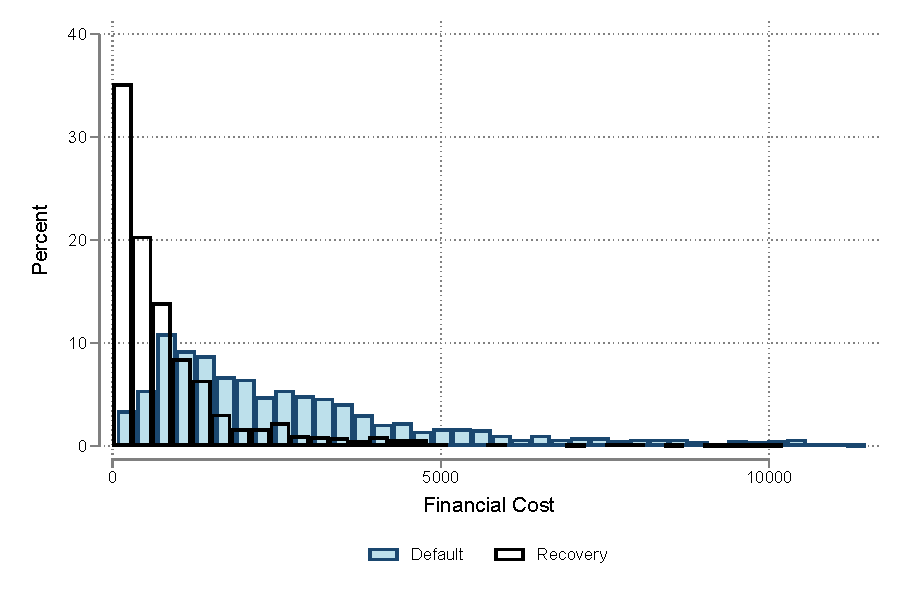
\includegraphics[width=\textwidth]{Figuras/hist_fc_0_0.pdf}
    \end{subfigure}
     \begin{subfigure}{0.45\textwidth}
    \caption{Effective APR (Ctrl = 0 Cmmtmnt = 0)}
       \centering
      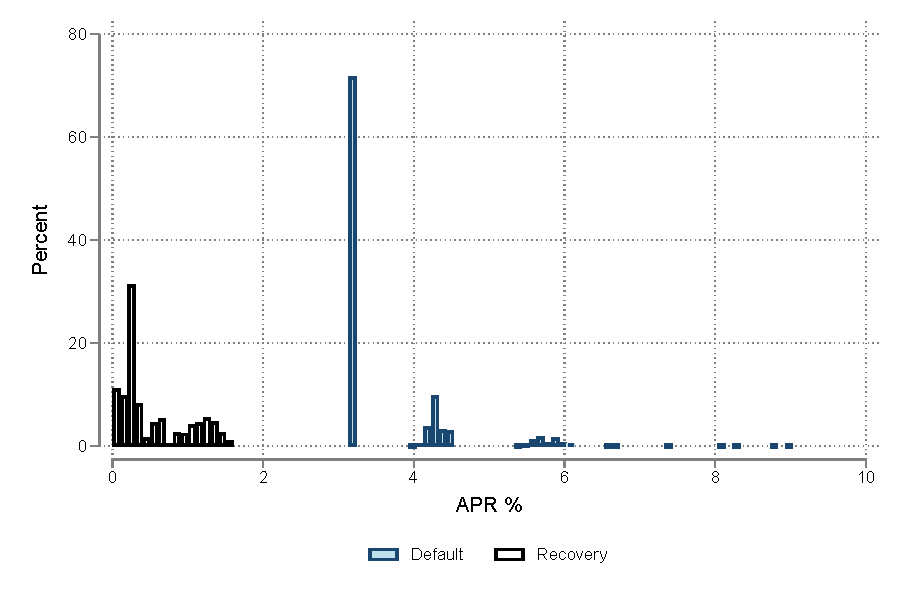
\includegraphics[width=\textwidth]{Figuras/hist_apr_0_0.pdf}
    \end{subfigure}
   \begin{subfigure}{.45\textwidth}
      \caption{FC (Ctrl = 0 Cmmtmnt = 1)}
        \centering
        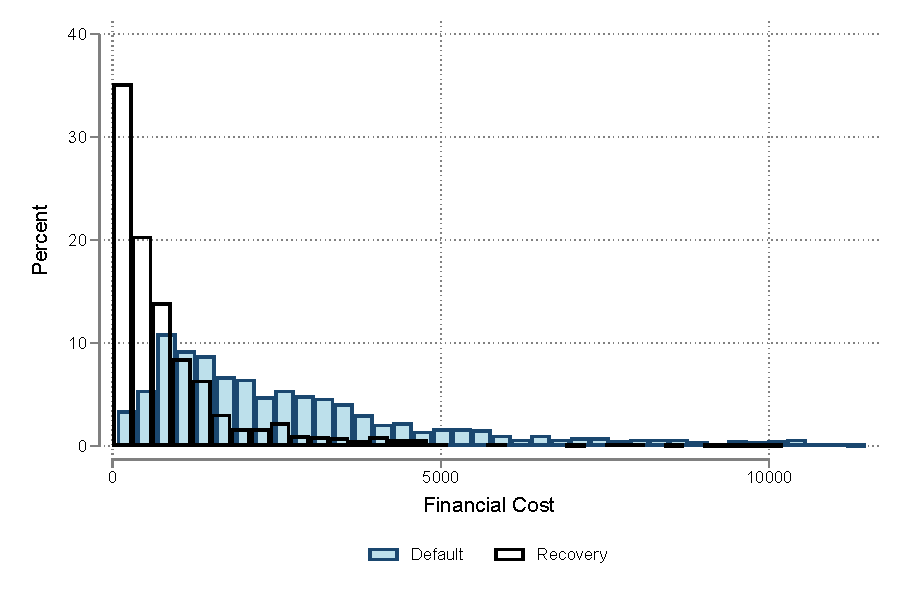
\includegraphics[width=\textwidth]{Figuras/hist_fc_0_1.pdf}
    \end{subfigure}
     \begin{subfigure}{0.45\textwidth}
    \caption{Effective APR (Ctrl = 0 Cmmtmnt = 1)}
       \centering
      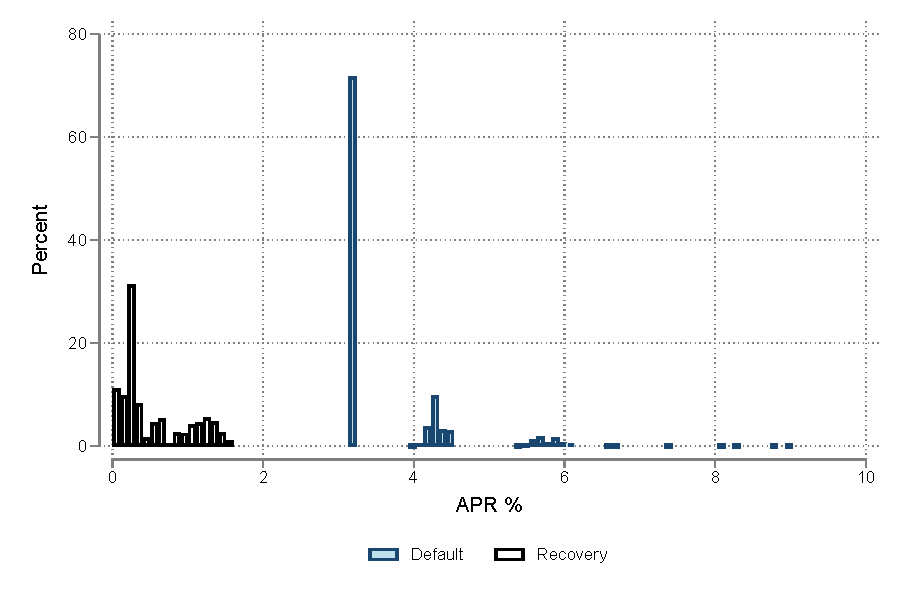
\includegraphics[width=\textwidth]{Figuras/hist_apr_0_1.pdf}
    \end{subfigure}
   \begin{subfigure}{.45\textwidth}
      \caption{FC (Ctrl = 1 Cmmtmnt = 0)}
        \centering
        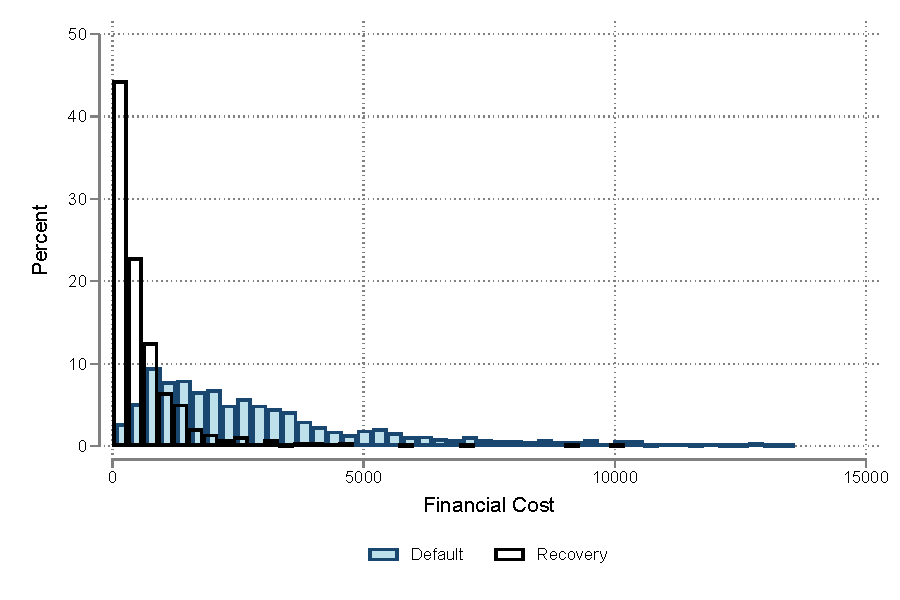
\includegraphics[width=\textwidth]{Figuras/hist_fc_1_0.pdf}
    \end{subfigure}
     \begin{subfigure}{0.45\textwidth}
    \caption{Effective APR (Ctrl = 1 Cmmtmnt = 0)}
       \centering
      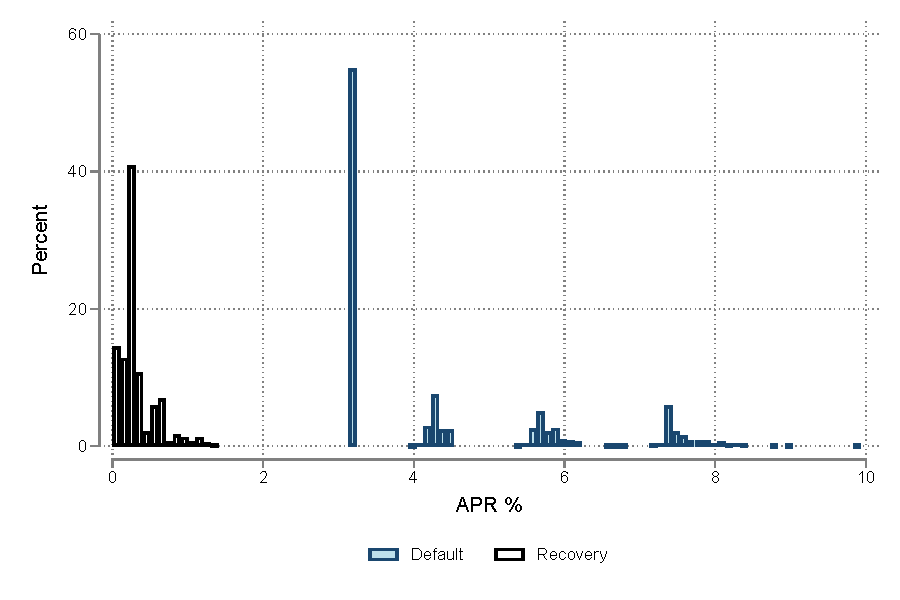
\includegraphics[width=\textwidth]{Figuras/hist_apr_1_0.pdf}
    \end{subfigure}
   \begin{subfigure}{.45\textwidth}
      \caption{FC (Ctrl = 1 Cmmtmnt = 1)}
        \centering
        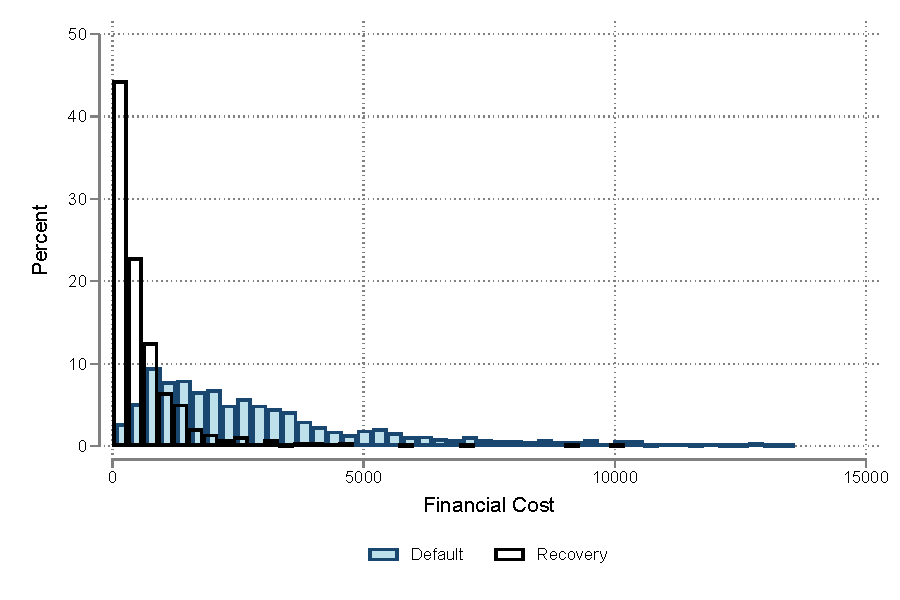
\includegraphics[width=\textwidth]{Figuras/hist_fc_1_1.pdf}
    \end{subfigure}
     \begin{subfigure}{0.45\textwidth}
    \caption{Effective APR (Ctrl = 1 Cmmtmnt = 1)}
       \centering
      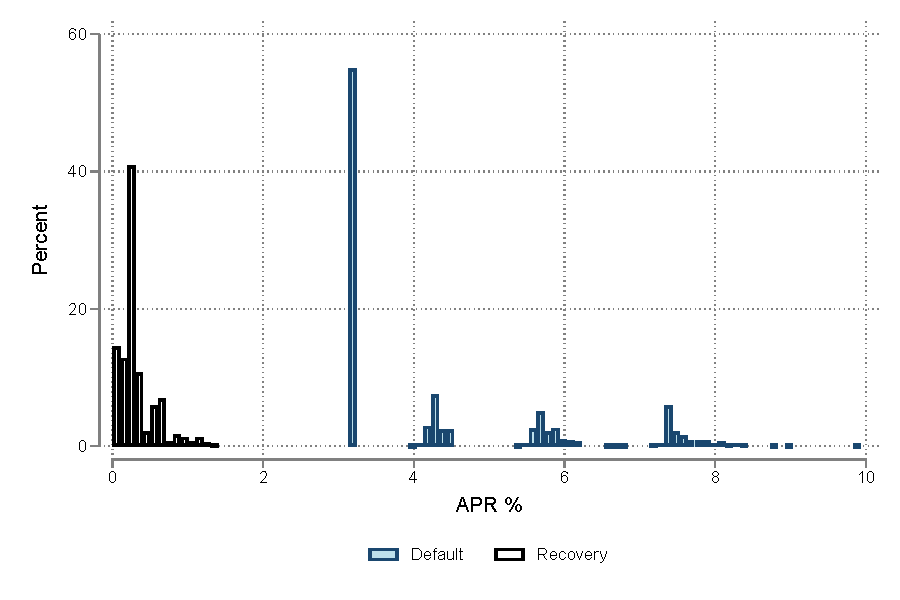
\includegraphics[width=\textwidth]{Figuras/hist_apr_1_1.pdf}
    \end{subfigure}    
    \end{center}
        
\end{figure}


\begin{table}[H]
\caption{Main results without censoring }
\label{mns}
\begin{center}
\scriptsize{% Table generated by Excel2LaTeX from sheet 'censoring_imp'
\begin{tabular}{lcccccc}
\toprule
      & FC    & Interest pymnt & Principal pymnt & Lost pawn value & Default & APR \\
\midrule
      & \multicolumn{6}{c}{Panel A : $\quad$ Control  = 0           $\quad\quad$                  Forced Commitment = 0} \\
\midrule
\midrule
      & (1)   & (2)   & (3)   & (4)   & (5)   & (6) \\
\midrule
\midrule
Forced commitment  & -236.0*** & -191.7*** & -0.63 & -75.9** & -0.064*** & -0.14*** \\
      & (48.1) & (37.6) & (3.01) & (30.5) & (0.023) & (0.022) \\
      &       &       &       &       &       &  \\
\midrule
Observations & 3724  & 3724  & 3724  & 3724  & 3724  & 3724 \\
R-sq  & 0.016 & 0.025 & 0.004 & 0.012 & 0.019 & 0.043 \\
Control Mean & 989.9 & 593.4 & 5.96  & 396.5 & 0.44  & 0.61 \\
\midrule
\midrule
      &       &       &       &       &       &  \\
\midrule
      & \multicolumn{6}{c}{Panel B : $\quad$ Control  = 0         $\quad\quad$                    Forced Commitment = 1} \\
\midrule
\midrule
      & (7)   & (8)   & (9)   & (10)  & (11)  & (12) \\
\midrule
\midrule
Forced commitment  & -191.2*** & -207.7*** & 1.17  & -15.1 & 0.0083 & -0.076*** \\
      & (49.7) & (37.4) & (3.45) & (31.2) & (0.024) & (0.026) \\
      &       &       &       &       &       &  \\
\midrule
Observations & 3724  & 3724  & 3724  & 3724  & 3724  & 3724 \\
R-sq  & 0.013 & 0.026 & 0.004 & 0.009 & 0.014 & 0.023 \\
Control Mean & 989.9 & 593.4 & 5.96  & 396.5 & 0.44  & 0.61 \\
\midrule
\midrule
      &       &       &       &       &       &  \\
\midrule
      & \multicolumn{6}{c}{Panel C : $\quad$ Control  = 1        $\quad\quad$                     Forced Commitment = 0} \\
\midrule
\midrule
      & (13)  & (14)  & (15)  & (16)  & (17)  & (18) \\
\midrule
\midrule
Forced commitment  & -319.0*** & -140.4*** & -2.33 & -210.3*** & -0.21*** & -0.24*** \\
      & (50.9) & (34.1) & (3.16) & (30.3) & (0.023) & (0.027) \\
      &       &       &       &       &       &  \\
\midrule
Observations & 3724  & 3724  & 3724  & 3724  & 3724  & 3724 \\
R-sq  & 0.021 & 0.020 & 0.004 & 0.021 & 0.053 & 0.061 \\
Control Mean & 1069.2 & 545.9 & 7.69  & 523.3 & 0.57  & 0.70 \\
\midrule
\midrule
      &       &       &       &       &       &  \\
\midrule
      & \multicolumn{6}{c}{Panel D : $\quad$ Control  = 1       $\quad\quad$                      Forced Commitment = 1} \\
\midrule
\midrule
      & (19)  & (20)  & (21)  & (22)  & (23)  & (24) \\
\midrule
\midrule
Forced commitment  & -274.2*** & -156.3*** & -0.53 & -149.6*** & -0.13*** & -0.17*** \\
      & (52.5) & (33.8) & (3.58) & (31.1) & (0.024) & (0.030) \\
      &       &       &       &       &       &  \\
\midrule
Observations & 3724  & 3724  & 3724  & 3724  & 3724  & 3724 \\
R-sq  & 0.017 & 0.021 & 0.003 & 0.013 & 0.028 & 0.032 \\
Control Mean & 1069.2 & 545.9 & 7.69  & 523.3 & 0.57  & 0.70 \\
\midrule
\midrule
      &       &       &       &       &       &  \\
\midrule
      & \multicolumn{6}{c}{Panel E : $\quad$ Prediction with lasso-logit model} \\
\midrule
\midrule
      & (25)  & (26)  & (27)  & (28)  & (29)  & (30) \\
\midrule
\midrule
Forced commitment  & -264.9*** & -169.6*** & -1.43 & -127.4*** & -0.12*** & -0.17*** \\
      & (53.8) & (37.2) & (3.52) & (33.1) & (0.025) & (0.028) \\
Choice commitment & -42.4 & -29.1 & -2.66 & -14.6 & -0.017 & 0.0026 \\
      & (56.9) & (41.8) & (3.24) & (34.9) & (0.024) & (0.029) \\
      &       &       &       &       &       &  \\
\midrule
Observations & 6304  & 6304  & 6304  & 6304  & 6304  & 6304 \\
R-sq  & 0.018 & 0.022 & 0.002 & 0.010 & 0.016 & 0.042 \\
Control Mean & 1034.5 & 563.4 & 7.69  & 471.2 & 0.52  & 0.66 \\
\bottomrule
\bottomrule
\end{tabular}%
}
\end{center}
 \scriptsize 
%\textit{Do file: } \texttt{tot\_tut.do}
\end{table}


\begin{table}[H]
\caption{ToT \& TuT with imputation}
\label{mns}
\begin{center}
\scriptsize{% Table generated by Excel2LaTeX from sheet 'tot_tut_imp'
\begin{tabular}{lccc}
\toprule
      & APR \% benefit & FC benefit & \% Recovery \\
\midrule
      & (1)   & (2)   & (3) \\
\midrule
\midrule
ATE   & 55.7*** & 510.0*** & 11.7*** \\
      & (11.2) & (123.5) & (2.57) \\
ToT   & 7.38  & 194.4 & 22.1 \\
      & (112.1) & (1252.7) & (22.2) \\
TuT   & 61.5*** & 547.7*** & 10.5*** \\
      & (13.0) & (130.0) & (2.71) \\
$\mathbb{E}[Y_1]$ & -227.7*** & -2073.6*** & 49.0*** \\
      & (7.73) & (74.5) & (1.85) \\
$\mathbb{E}[Y_0]$ & -172.0*** & -1563.6*** & 60.7*** \\
      & (8.06) & (98.5) & (1.79) \\
\midrule
ToT-TuT & -54.1 & -353.3 & 11.6 \\
      & (119.7) & (1324.7) & (23.5) \\
ASB   & 53.5  & 661.6 & -15.7 \\
      & (118.2) & (1320.1) & (23.2) \\
ASL   & -0.63 & 308.3* & -4.09 \\
      & (19.2) & (169.0) & (4.49) \\
      &       &       &  \\
\midrule
Observations & 6304  & 6304  & 6304 \\
Control Mean & -227.7 & -2073.6 & 49.0 \\
$H_0$ : ATE-TuT=0 & 0.65  & 0.79  & 0.62 \\
$H_0$ : ATE-ToT=0 & 0.65  & 0.79  & 0.62 \\
$H_0$ : ToT-TuT=0 & 0.65  & 0.79  & 0.62 \\
$H_0$ : ToT-TuT$\geq$ 0 & 0.67  & 0.61  & 0.31 \\
\bottomrule
\bottomrule
\end{tabular}%
}
\end{center}
 \scriptsize 
%\textit{Do file: } \texttt{tot\_tut.do}
\end{table}

\end{document}
